\section{Fondamenti teorici}
\subsection{Hierarchical Model Reduction in 3D}
 \begin{frame}
  \frametitle{Motivazione}
  \framesubtitle{esistenza di una direzione dominante}
  \begin{exampleblock}{}
 Vogliamo risolvere un certo tipo di problemi: quelli che presentano una direzione preferenziale
\begin{center}
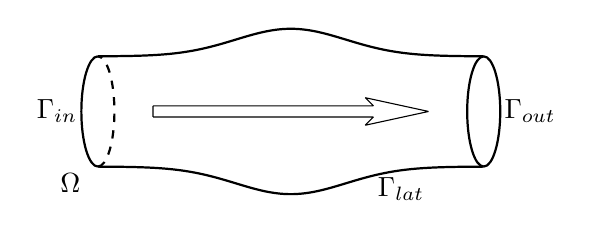
\begin{tikzpicture}
[scale=0.7]
\def\xi{0};
\def\xo{7};
\def\c{3.5};
\def\r{1};
\def\sig{2};
\def\rmax{0.5};
\def\rtot{\rmax+\r};
\def\yd{-0.1}
\def\yu{-\yd}
\def\xs{1}
\def\xf{5}
\def\xe{6}
\def\xa{0.15}
\def\ya{0.15}
 \draw (\xs,\yd) -- (\xf,\yd)
       (\xf,\yd) -- (\xf-\xa,\yd-\ya)
       (\xf-\xa,\yd-\ya) -- (\xe,0)
       (\xe,0) -- (\xf-\xa,\yu + \ya)
       (\xf-\xa,\yu + \ya) -- (\xf,\yu)
       (\xf,\yu) -- (\xs,\yu)
       (\xs,\yu) -- (\xs,\yd);
\draw[thick] (\xi,\r) arc (90:270:0.3cm and \r cm);
\draw[dashed,thick] (\xi,-\r) arc (-90:90:0.3cm and \r cm);

\draw[thick] (\xo,\r) arc (90:270:0.3cm and \r cm);
\draw[thick] (\xo,-\r) arc (-90:90:0.3cm and \r cm);

\draw[thick,parametric,domain=-\xi:\xo,samples=200,variable=\t] plot ({\t},{\r+\rmax*exp{-pow(\t-\c,2)/\sig}});
\draw[thick,parametric,domain=-\xi:\xo,samples=200,variable=\t] plot ({\t},{-\r-\rmax*exp{-pow(\t-\c,2)/\sig}});
\def\po{0.9};
\node[left] at(\xi-0.2,0) {$\Gamma_{in}$};
\node[right] at(\xo +0.2,0) {$\Gamma_{out}$};
\node at (\xi -0.5,-1.3) {$\Omega$};
\node at (\c +2,-\r-0.4) {$\Gamma_{lat}$};
\end{tikzpicture}
\end{center}
\end{exampleblock}
\begin{center}
\tikzstyle{3d} = [ellipse, draw, fill=red!50, 
    text width=7em,text badly centered, inner sep=0pt]

\tikzstyle{1d} = [ellipse, draw, fill=blue!30, 
    text width=7em,text badly centered, inner sep=0pt]
    
\tikzstyle{himod} = [rectangle, draw, fill=blue!50!red!50!white]
\begin{tikzpicture}
\def\x{7};
\node[1d] (1d) at (0,0) {\textbf{Modello 1D}\\{\footnotesize Bassa precisione}\\{\footnotesize Economico}};
\node[3d] (3d) at (\x,0) {\textbf{Modello 3D}\\{\footnotesize Alta precisione}\\{\footnotesize Costoso}};
\node[himod] (himod) at (\x/2,0) {HiMod};
\path[draw,thick,dashed,->] (1d) -- (himod);
\path[draw,thick,dashed,<-] (himod) -- (3d);

			  
%smily face sinistra
\def\f{1.0}
\def\alt{-0.5}
\def\rad{0.15}
\draw[thin] (\f,\alt) circle(\rad cm);
\draw[thin] plot [smooth,tension=1.5] coordinates{(\f - 0.5*\rad,\alt - 0.4*\rad) (\f + 0*\rad,\alt - 0.7*\rad) (\f + 0.5*\rad,\alt -0.4*\rad)};
% \draw[thin, fill=black] (\f+0*\rad,\alt-0.2*\rad) circle (0.1*\rad);
\draw[thin] plot [smooth,tension=1.5] coordinates{(\f-0.4*\rad,\alt+0.4*\rad) (\f-0.3*\rad,\alt +0.5*\rad) (\f-0.2*\rad,\alt+0.4*\rad)};
\draw[thin] plot [smooth,tension=1.5] coordinates{(\f+0.4*\rad,\alt+0.4*\rad) (\f+0.3*\rad,\alt+0.5*\rad) (\f+0.2*\rad,\alt+0.4*\rad)};

  
%smily face sinistra
\def\f{8.25}
\def\alt{-0.05}
\def\rad{0.15}
\draw[thin] (\f,\alt) circle(\rad cm);
\draw[thin] plot [smooth,tension=1.5] coordinates{(\f - 0.5*\rad,\alt - 0.4*\rad) (\f + 0*\rad,\alt - 0.7*\rad) (\f + 0.5*\rad,\alt -0.4*\rad)};
% \draw[thin, fill=black] (\f+0*\rad,\alt-0.2*\rad) circle (0.1*\rad);
\draw[thin] plot [smooth,tension=1.5] coordinates{(\f-0.4*\rad,\alt+0.4*\rad) (\f-0.3*\rad,\alt +0.5*\rad) (\f-0.2*\rad,\alt+0.4*\rad)};
\draw[thin] plot [smooth,tension=1.5] coordinates{(\f+0.4*\rad,\alt+0.4*\rad) (\f+0.3*\rad,\alt+0.5*\rad) (\f+0.2*\rad,\alt+0.4*\rad)};

  
%sad face destra
\def\f{7.8}
\def\alt{-0.5}
\def\rad{0.15}
\draw[thin] (\f,\alt) circle(\rad cm);
\draw[thin] plot [smooth,tension=1.5] coordinates{(\f-0.3*\rad,\alt-0.6*\rad) (\f-0.2*\rad,\alt-0.5*\rad) (\f +0.3*\rad,\alt-0.5*\rad)};
\draw[thin] (\f-0.4*\rad,\alt+0.4*\rad) -- (\f-0.2*\rad,\alt +0.3*\rad);
\draw[thin] (\f+0.4*\rad,\alt+0.5*\rad) -- (\f+0.2*\rad,\alt +0.4*\rad);
% \draw[thin, fill=black] (\f+0*\rad,\alt-0.2*\rad) circle (0.1*\rad);
%sad face sinistra
\def\f{1.4}
\def\alt{-0.05}
\def\rad{0.15}
\draw[thin] (\f,\alt) circle(\rad cm);
\draw[thin] plot [smooth,tension=1.5] coordinates{(\f-0.3*\rad,\alt-0.6*\rad) (\f-0.2*\rad,\alt-0.5*\rad) (\f +0.3*\rad,\alt-0.5*\rad)};
\draw[thin] (\f-0.4*\rad,\alt+0.4*\rad) -- (\f-0.2*\rad,\alt +0.3*\rad);
\draw[thin] (\f+0.4*\rad,\alt+0.5*\rad) -- (\f+0.2*\rad,\alt +0.4*\rad);
% \draw[thin, fill=black] (\f+0*\rad,\alt-0.2*\rad) circle (0.1*\rad);
\end{tikzpicture}
\end{center}
 \end{frame}

 \begin{frame}
 \frametitle{Impostazione geometrica}
 \framesubtitle{il dominio}
 
\begin{itemize}
 \item Fibra di supporto rettilinea \textcolor{blue}{$\Omega_{1D}$} dove avviene la dinamica dominante.
 \item Suddivisione del dominio in slices \textcolor{red}{$\gamma_x$} ortogonali alla fibra di supporto.
\end{itemize}

$$\Omega=\bigcup_{x\in\Omega_{1D}}\gamma_x$$
\begin{center}
\begin{tikzpicture}
[scale=0.8]
\def\xi{0};
\def\xo{7};
\def\c{3.5};
\def\r{1};
\def\sig{2};
\def\rmax{0.5};
\def\rtot{\rmax+\r};

\draw[thick] (\xi,0) arc (90:270:0.3cm and \r cm);
\draw[dashed,thick] (\xi,-2*\r) arc (-90:90:0.3cm and \r cm);

\draw[thick] (\xo,0) arc (90:270:0.3cm and \r cm);
\draw[thick] (\xo,-2*\r) arc (-90:90:0.3cm and \r cm);

% \draw[->] (-2,0) -- (2,0);
% \draw[->] (0,-2) -- (0,2);
\draw[thick,parametric,domain=-\xi:\xo,samples=200,variable=\t] plot ({\t},{\rmax*exp{-pow(\t-\c,2)/\sig}});
\draw[thick,parametric,domain=-\xi:\xo,samples=200,variable=\t] plot ({\t},{-2*\r-\rmax*exp{-pow(\t-\c,2)/\sig}});
\draw[thick,parametric,domain=-\xi:\xo,samples=200,variable=\t,dashed,blue] plot ({\t},{-\r});
\draw[color=red!70,pattern=north west lines, pattern color=red!20, thick] (\c,-\r) ellipse (0.3 and \rtot);
\def\po{0.9};
\node[below,blue] at (\xo*\po,-\r) {$\Omega_{1D}$};
\node[below,red] at (\c,-2*\r-\rmax) {$\gamma_x$};
\node[left] at(\xi-0.2,-\r) {$\Gamma_{in}$};
\node[right] at(\xo +0.2,-\r) {$\Gamma_{out}$};
\node at (\xi -0.5,-\r-1.3) {$\Omega$};
\node at (\c +2,-2*\r-0.4) {$\Gamma_{lat}$};
\end{tikzpicture}
\end{center}
\end{frame}

 \begin{frame}
 \frametitle{Processo di riduzione}
 \framesubtitle{mapping e serie di Fourier}
 Idea: 
 \begin{itemize}
  \item mappare $\Omega$ in un dominio di riferimento $\widehat \Omega$ in modo che $$\hat \gamma_{\hat x}=\hat \gamma\,\,\forall \hat x\in\widehat\Omega_{1D}$$
  \item espandere, in direzione trasversale, la soluzione rispetto alla base di Fourier generalizzata $$\{\varphi_k(y,z)\}_{k\in\mathbb{N}}$$
 \end{itemize}
 Noi lavoreremo direttamente in un riferimento, quindi non utilizzeremo la notazione con i cappelli.
 \begin{block}{Spazi in direzione trasversale}
 \footnotesize
  $$V^\infty_\gamma=\left\{v(y,z)=\sum_{k=1}^\infty v_k\varphi_k(y,z)\right\}$$
  $$V^m_\gamma=\left\{v(y,z)=\sum_{k=1}^m v_k\varphi_k(y,z)\right\}$$
 \end{block}
 \end{frame}
\begin{frame}
 \frametitle{Processo di riduzione}
 \framesubtitle{Spazi ridotti}
 Lungo la direzione principale usiamo uno spazio $V_{1D}$ di tipo $H^1(\Omega_{1D})$ che consideri correttamente le condizioni al bordo.
 Possiamo ora definire gli spazi ridotti come spazi prodotto:
 \begin{block}{Spazi ridotti}
  $$V^\infty(\Omega)=V_{1D}\otimes V^\infty_\gamma:=\left\{v(x,y,z)=\sum_{k=1}^\infty v_k(x)\varphi_k(y,z), v_k\in V_{1D}\right\}.$$
  $$V^m(\Omega)=V_{1D}\otimes V^m_\gamma:=\left\{v(x,y,z)=\sum_{k=1}^m v_k(x)\varphi_k(y,z), v_k\in V_{1D}\right\}.$$
  \end{block}
\end{frame}
% \begin{frame}
%  \frametitle{Spazi prodotto}
%  \framesubtitle{Alcune propriet\`a}
%  \begin{itemize}
%   \item $V^{\infty}(\Omega)$ \`e l'insieme delle combinazioni lineari delle funzioni di base sulla slice trasversale, con coefficienti che sono
%   a loro volta funzioni di $V_{1D}$.
%   \item \`E possibile mostrare che $V^{\infty}(\Omega)$ \`e isometricamente isomorfo a $H^1_D(\Omega)$
%  \end{itemize}
% 
% \end{frame}


 \begin{frame}
  \frametitle{Modelli ridotti}
  \framesubtitle{Problemi 1D accoppiati}
  una equazione tipo questa
  pi\`u qualche spiegazione
  {\footnotesize
\begin{equation}
\label{eq:modalreducedcoeff}
 \sum_{k=1}^m\int_{\Omega_{1D}}
 \biggl[
 \underbrace{\hat r^{11}_{k,j}\dpar{\hat u_k}{\xhat}\dpar{\theta}{\xhat}}_{\text{Diffusion}}
+\underbrace{\hat r^{10}_{k,j}\dpar{\hat u_k}{\xhat}\theta}_{\text{Advection}}
+\underbrace{\hat r^{01}_{k,j}\hat u_k\dpar{\theta}{\xhat}}_{\text{One-order term}}
+\underbrace{\hat r^{00}_{k,j}\hat u_k\theta}_{\text{Reaction}}
d\xhat\biggr]=\int_{\Omega_{1D}}\nsp{8}\theta\hat f_k d\xhat.
\end{equation}}
 \end{frame}

\begin{frame}
 \frametitle{Basis choice}
 \framesubtitle{The sinusoidal basis}
 \begin{itemize}
  \item Letteratura: in perotto:2008, dirichlet, base di soli seni (2D).
  \item Letteratura: legendre polynomials x $(1-x^2)$.
  \item Educated basis x condizioni al bordo pi\`u generali.
 \end{itemize}
\end{frame}

 
\subsection{Basi istruite}
\begin{frame}
  \frametitle{Base teorica}
  \framesubtitle{Teorema spettrale per forme bilineari}
  \begin{itemize}
   \item teorema spettrale solito (salsa)
  \end{itemize}

 \end{frame}
 
\begin{frame}
 \frametitle{Ipotesi geometriche}
 \framesubtitle{Dominio parallelepipedo}
 \begin{center}
\begin{tikzpicture}
[scale=1.5]

\draw [thick] (2,0) rectangle (3,1);
\node at (-0.25,1.25) {$\Gamma_{in}$};
\node at (3.3,0.5) {$\Gamma_{out}$};
\node at (2,1.75) {$\Gamma_{vaso}$};
\node at (0.5,0.4) {$\gamma$};
% \node at (0.7,0.88) {$\gamma}$};
\node at (3.5,-0.2) {$\Omega_{1D}$};


\draw [thick] (2,1)--(0,2)--(1,2)--(3,1);
\draw [thick] (2,0)--(0,1)--(0,2);

\draw [dashed,thick] (0,1)--(1,1)--(1,2);
\draw [dashed,thick] (1,1)--(3,0);

\draw [pattern=north west lines, pattern color=gray, thick] (0.5,0.75) rectangle (1.5,1.75);

\draw [thick,dashed, ->] (-0.5,2)--(3.5,0);

\end{tikzpicture}
\end{center}
 \begin{itemize}
  \item si pu\`o fare anche con il cerchio
  \item condizioni al bordo a coefficienti costanti su ogni lato del quadrato
 \end{itemize}
\end{frame}


\begin{frame}
 \frametitle{Separazione di variabili}
 \framesubtitle{Due sottoproblemi agli autovalori}
 \begin{itemize}
 \item i conti
 \item la tabella con i risultati
 \end{itemize}
\end{frame}

\begin{frame}
 \frametitle{Un problema di ordinamento}
 \framesubtitle{Esempio caso condizioni di Dirichlet}
 
 facciamo qui un esempio numerico con Ly diverso da Lz e i conti proprio
 questa ultima slide ci da il la per la seconda sezione
\end{frame}